\documentclass[11pt]{amsart}
\usepackage{geometry}                % See geometry.pdf to learn the layout options. There are lots.
\geometry{letterpaper}                   % ... or a4paper or a5paper or ... 
%\geometry{landscape}                % Activate for for rotated page geometry
%\usepackage[parfill]{parskip}    % Activate to begin paragraphs with an empty line rather than an indent
\usepackage{graphicx}
\usepackage{subfigure}
\usepackage{amssymb}
\usepackage{epstopdf}
\DeclareMathOperator*{\argminA}{arg\,min} % Jan Hlavacek
\DeclareMathOperator*{\argminB}{argmin}   % Jan Hlavacek
\DeclareMathOperator*{\argminC}{\arg\min}   % rbp

\newcommand{\argminD}{\arg\!\min} % AlfC

\newcommand{\argminE}{\mathop{\mathrm{argmin}}}          % ASdeL
\newcommand{\argminF}{\mathop{\mathrm{argmin}}\limits}   % ASdeL

% limits on side
\DeclareMathOperator{\argminG}{arg\,min} % Jan Hlavacek
\DeclareMathOperator{\argminH}{argmin}   % Jan Hlavacek
\newcommand{\argminI}{\mathop{\mathrm{argmin}}\nolimits} % ASdeL

\newcommand{\cs}[1]{\texttt{\symbol{`\\}#1}}
\DeclareGraphicsRule{.tif}{png}{.png}{`convert #1 `dirname #1`/`basename #1 .tif`.png}
\geometry{left=2cm,right=2cm}
\title{ Reinforcement learning in financial computing}
%\author{The Author}
%\date{}                                           % Activate to display a given date or no date

\begin{document}
\maketitle
%\section{}
%\subsection{}

\section{Problem}
When we train a neural network, how to avoid local minimum is always a classical problem. Different situations may correspond to different problems. For our neural network, we repeatedly fall into the local minimum similar to the following picture.

\begin{figure}[ht]
 
\centering
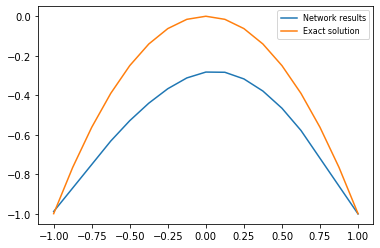
\includegraphics[scale=0.5]{result1.jpg}
\caption{Result trained by our original design with max norm error about 26$\%$}
\label{figl}
 
\end{figure}

We tried many ways to reduce the loss but failed and then we focused on the source of loss. As we mentioned before, compared with value iteration, our model uses the parameters of neural network instead of the original grid to record the information so our loss is the sum of the losses of all points. From the above results, obviously, most of the error with exact solution comes from the middle point. However, from the perspective of loss function, the problem is totally different.

\begin{figure}[ht]
 
\centering
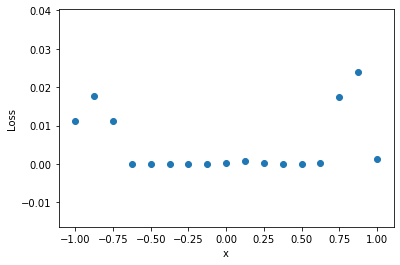
\includegraphics[scale=0.5]{local_minimum.jpg}
\caption{The loss in each point}
\label{figl}
 
\end{figure}

From the perspective of loss function, the losses in middle points are small and the most part of loss comes from the boundary and the points close to the boundary. In other words, for the middle points, the neural network thinks 'he' has done a good job. Since the values of middle points derived from the points close to the boundary, if the values of points close to the boundary have some error, the error of middle points will be larger. For value iteration, it is not a problem, there is a table to record the information of each point one by one. When the table is updating, each point's value can move in the best direction of itself. However, in our model, when we update the parameters of network, the loss function move in the best direction of the whole points where each points has the same weight. In this case, this direction may not be optimal for the points close to boundary which are more important. To solve the problem, I came up with two ways:
\begin{itemize}
 \item Given different weights to the losses generated by different points. But there is a new problem, how to define the weights? Just using the distance from the point to the boundary has been tried and failed.
 \item When we go into this local minimum, we can only update the points whose loss larger than a threshold.in mathematics:
$$
L(\theta,x_i) = 
\argminA_\theta\Big \{h(x,\theta) - \gamma \inf_{a} 
\Big\{ \ell^{h}(x, a) + 
\sum_{i=1}^{d} 
p^{h}(x+he_{i}|x, a) h(x+he_{i} ,\theta)
+ p^{h}(x-he_{i}|x, a) h(x-he_{i} ,\theta)\Big\}\Big\}
$$
$$
L(\theta) = \sum_{i=1}^{N}L(\theta,x_i) , L(\theta,x_i) > threshold
$$
And this is the result:
\begin{figure}[ht]
\centering
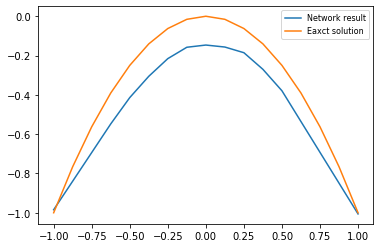
\includegraphics[scale=0.5]{result_trypng.jpg}
\caption{Add a threshold in loss function}
\label{figl}
\end{figure}
\begin{figure}[ht]
\centering
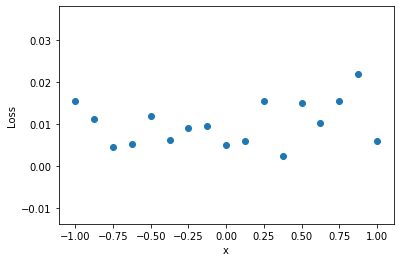
\includegraphics[scale=0.5]{problem1.jpg}
\caption{The loss in each point with threshold}
\label{figl}
\end{figure}
\end{itemize}
\end{document}  